\documentclass[12pt]{article}

\usepackage{amsmath}
\usepackage{unicode-math}
\usepackage{xltxtra}
\usepackage{xgreek}

\setmainfont{Liberation Serif}

\usepackage{tabularx}

\usepackage[table]{xcolor}
\usepackage{tikz}
\pagestyle{empty}

\usepackage{geometry}
 \geometry{a4paper, total={190mm,275mm}, left=10mm, top=10mm}

 \usepackage{graphicx}
 \graphicspath{ {images/} }

 \usepackage{wrapfig}
\usepackage{lipsum}%% a garbage package you don't need except to create examples.

\begin{document}
\part*{\centering{Πανελλήνιες Μαθηματικά Γ Λυκείου 2018 Λύσεις}}

\section*{Θέμα Β}
  \begin{enumerate}
    \item [B1.] Η συνάρτηση $f$ είναι συνεχής και παραγωγίσιμη για $x\in \mathbb{R}-{0}$. Η παράγωγός της είναι
    $$f'(x)=1+\frac{8}{x^3}$$
    Για $f'(x)=0 \Rightarrow x=-2$. Έτσι η συνάρτηση είναι για $x<-2$ γνήσια αύξουσα, για $-2<x<0$ γνήσια φθίνουσα και για $x>0$ γνήσια φθίνουσα. Το μοναδικό τοπικό ακρότατο λοιπόν είναι στο $x=-2$ με $f(-2)=-3$

    \item [B2.] Η δεύτερη παράγωγος της συνάρτησης είναι $f''(x)=-\frac{24}{x^4}<0$. Άρα η συνάρτηση είναι κοίλη για $x<0$ και επίσης κοίλη για $x>0$. Συνεπώς δεν υπάρχουν σημεία καμπής.

    \item [B3.] Για κατακόρυφη ασύμπτωτη έχουμε $\lim_{x\to 0}f(x)=-\infty$ άρα παρουσιάζεται κατακόρυφη η $x=0$. Για την πλάγια στο $+\infty$, έχουμε
    $$\lim_{x\to \infty}\frac{f{x}}{x}=\lim_{x\to \infty}1-\frac{4}{x^3}=1 $$
    και
    $$\lim_{x\to \infty} f(x)-x= -\lim_{x\to \infty}\frac{4}{x^2}=0$$
    άρα η πλάγια στο $+\infty$ είναι η $y=x$.
    Όμοια για το $-\infty$, έχουμε
    $$\lim_{x\to -\infty}\frac{f{x}}{x}=\lim_{x\to -\infty}1-\frac{4}{x^3}=1$$
    και
    $$\lim_{x\to -\infty} f(x)-x= -\lim_{x\to -\infty}\frac{4}{x^2}=0$$
    άρα η πλάγια στο $-\infty$ είναι η $y=x$.

    \item [B4.]

      Ο πίνακας μελέτης της συνάρτησης λοιπόν είναι ο:

      $$\begin{array}{c | c c c c c c c}
        x & -\infty & & -2 & & 0 & & +\infty \\ \hline
        φ'(x)  & & + & 0 & - & || & + &\\
        φ''(x) & & - & \vline & - & || & - & \\ \hline
        φ(x)   & & \begin{tikzpicture}[scale=0.5]\draw [->] (0,0) to[out=45,in=180](1,0.5);\end{tikzpicture} & & \begin{tikzpicture}[scale=0.5]\draw [->] (0,0) to[out=0,in=135](1,-0.5);\end{tikzpicture}  & || & \begin{tikzpicture}[scale=0.5]\draw [->] (0,0) to[out=45,in=180](1,0.5);\end{tikzpicture}
      \end{array}$$

      Η γραφική της παράσταση είναι η

      \begin{figure}
        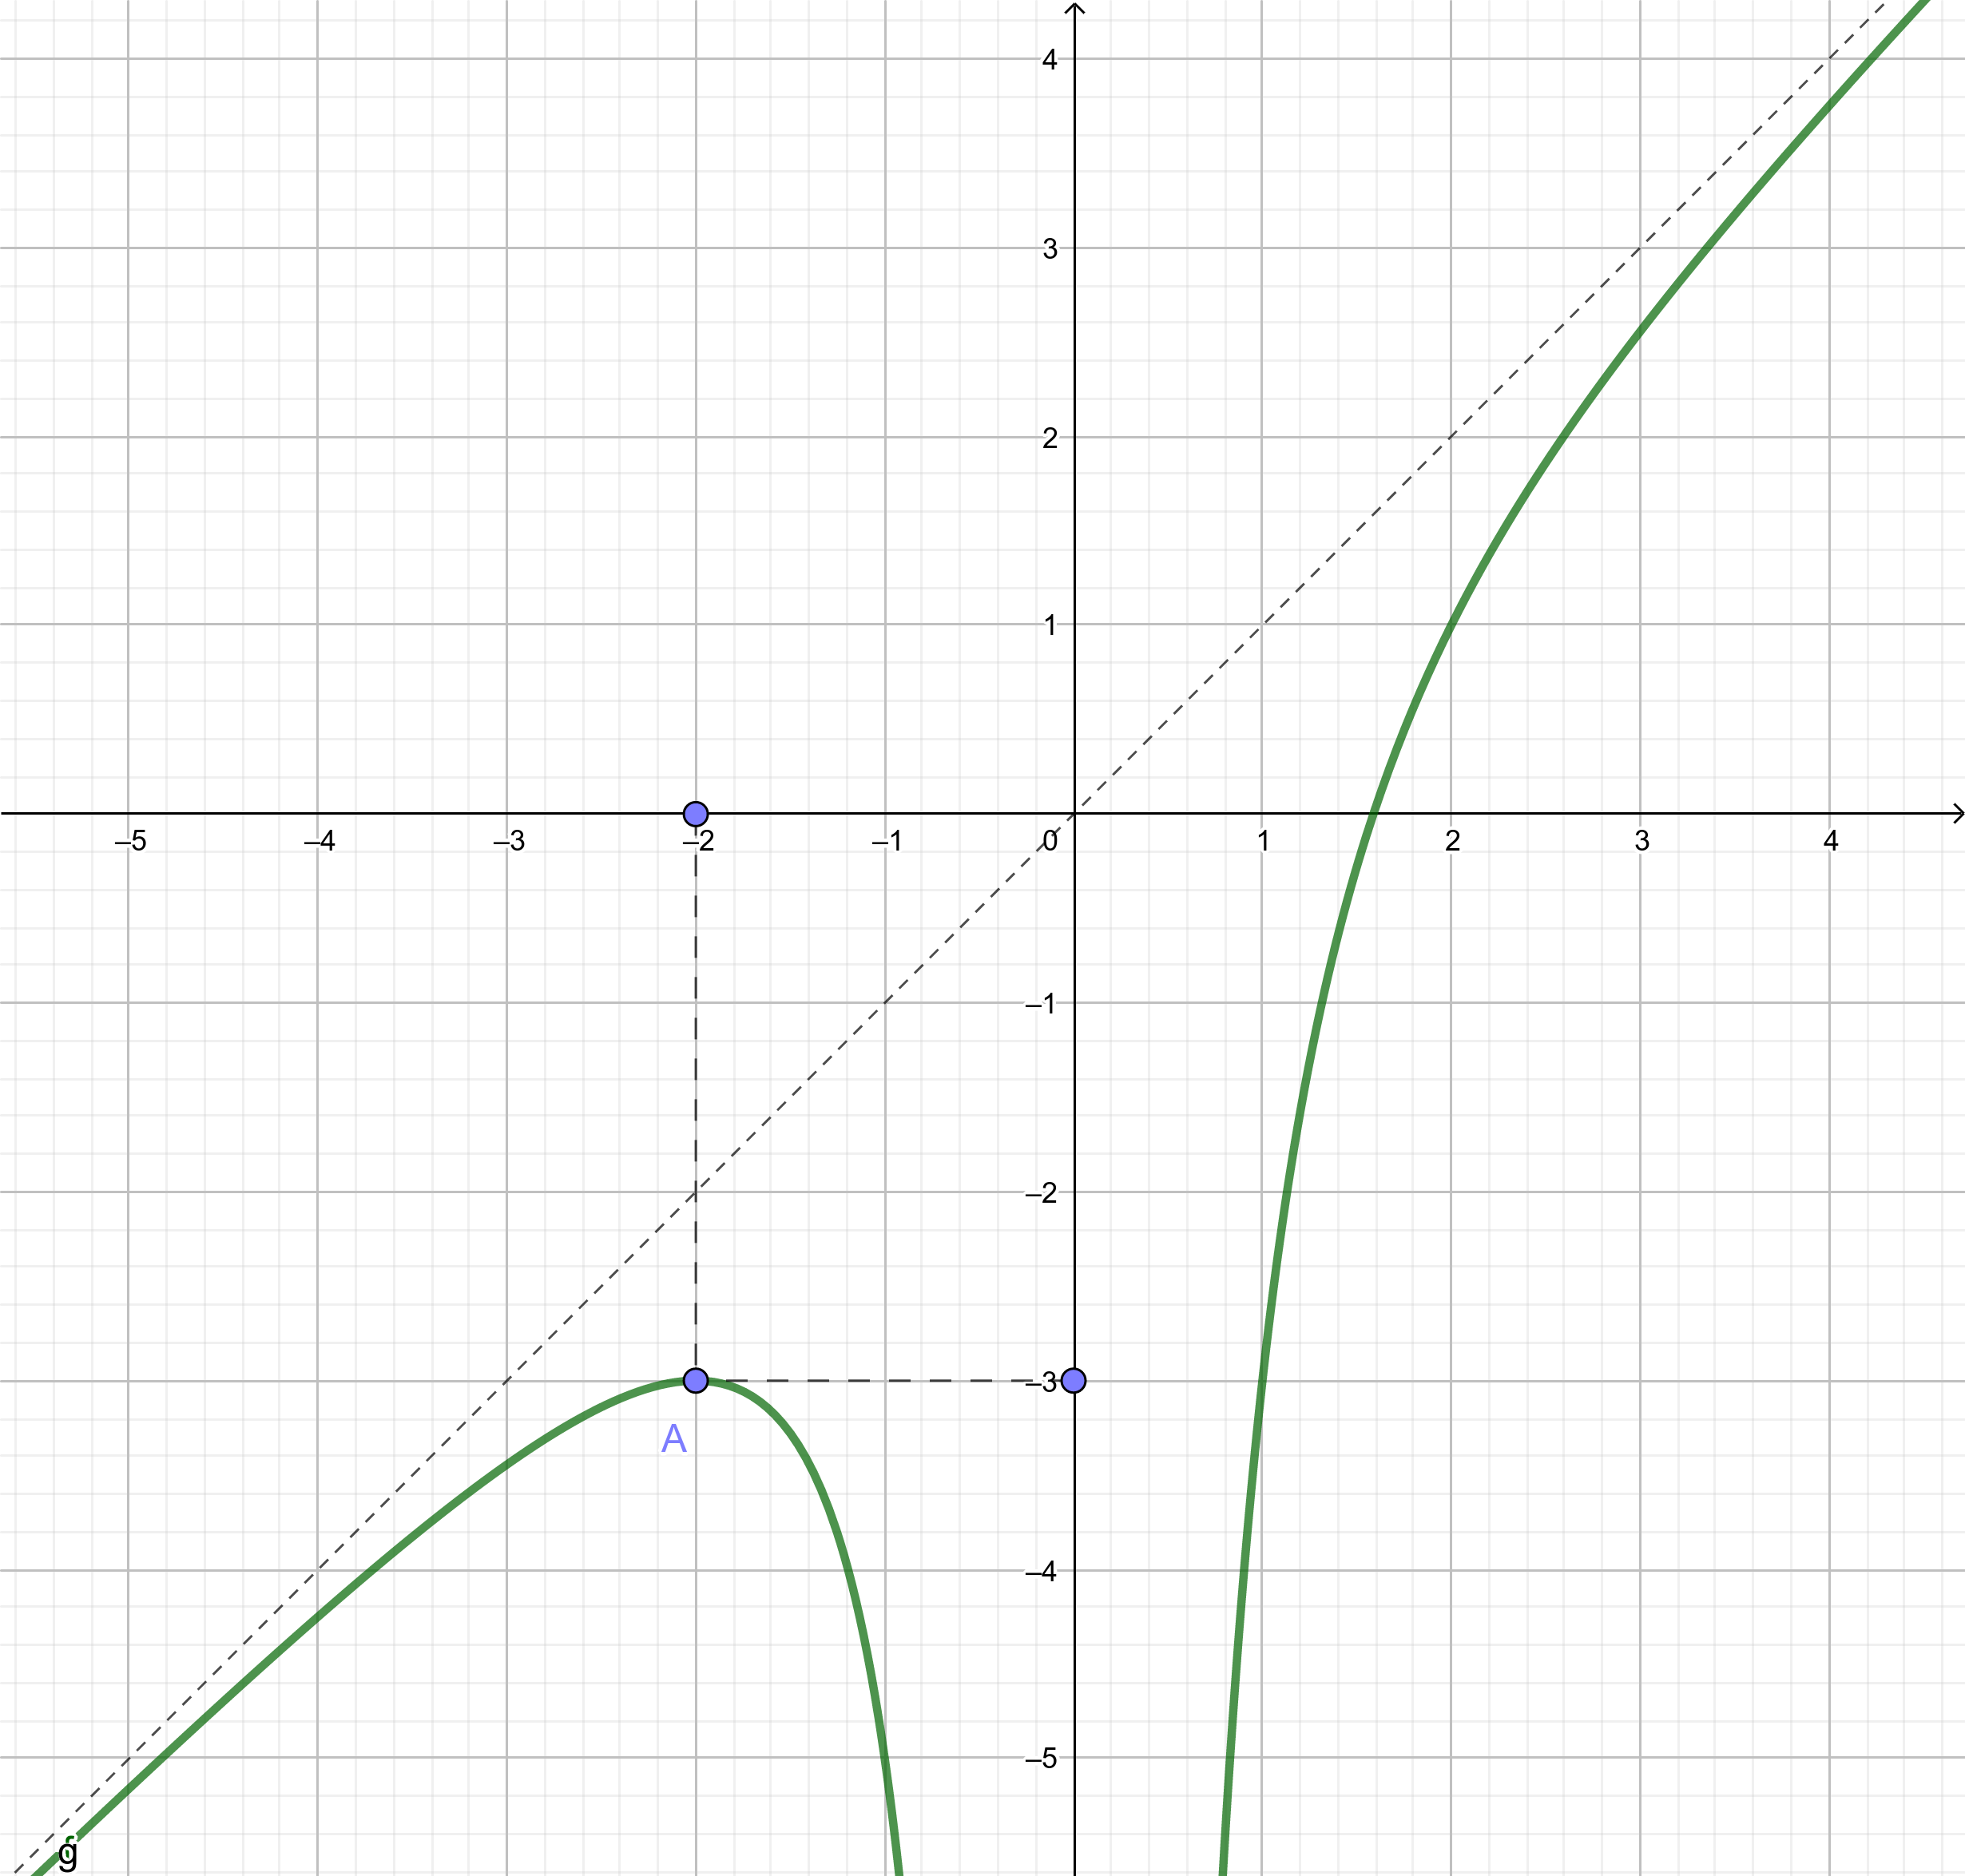
\includegraphics[width=0.25\textwidth]{2018PanelliniesΒ.png}
        \centering
      \end{figure}
  \end{enumerate}

  \section*{Θέμα Γ}
    \begin{enumerate}
      \item [Γ1.] Έστω $x$ το τμήμα για το τετράγωνο. Τότε η πλευρά του τετραγώνου θα είναι $\frac{x}{4}$ συνεπώς το εμβαδό του θα είναι $\frac{x^2}{16}$. Το υπόλοιπο τμήμα $8-x$ θα είναι η περίμετρος του κύκλου. Άρα $8-x=2πρ \Rightarrow ρ=\frac{8-x}{2π}$. Συνεπώς το εμβαδό του κύκλου θα είναι $πρ^2=\frac{(8-x)^2}{4π}$. Συνολικά το εμβαδό του σχήματος θα είναι
      $$Ε=\frac{x^2}{16}+\frac{(8-x)^2}{4π}=\cdots=\frac{(π+4)x^2-64x+256}{16π}$$


      \item [Γ2.] Η συνέρτηση $Ε(x)$ είναι παραγωγίσιμη με $Ε'(x)=\frac{2(π+4)x-64x}{16π}$. Έτσι είναι φθίνουσα για $x<\frac{32}{π+4}$ είναι αύξουσα για $x>\frac{32}{π+4}$. Στο $x=\frac{32}{π+4}$ παρουσιάζει ελάχιστο.

      \item [Γ3.] Για να λυθεί η εξίσωση $E(x)=5$ αρκεί να μελετήσουμε το σύνολο τιμών της $E(x)$. Παρατηρούμε ότι $E(0)=\frac{16}{π}>5$ και $E(8)=4<5$. Άρα στο πρώτο διάστημα $0<x<\frac{16}{π}$ υπάρχει μοναδικό $x_0$ ώστε $f(x_0)=5$ ενώ για $\frac{16}{π}<8<8$ η εξίσωση είναι αδύνατη.
      \item [Γ3.] Β Λύση Θα λυθεί η εξίσωση

    \begin{gather*}
      E(x)=5 \Rightarrow (π+4)x^2-64x+256-80π=0 \\\
      Δ=4096-4(π+4)(256-80π)=256π + 320π^2 \\\
      x_{1,2}=\frac{64\pm \sqrt{256π + 320π^2}}{2(π+4)}=\frac{4(8\pm \sqrt{5π^2+4π})}{π+4}
    \end{gather*}

    Θα πρέπει να βρούμε τις λύσεις που $0<x<8$. έχουμε

    \begin{gather*}
      3.1<π<3.2 \\\
      60,45<5π^2+4π<64 \\\
      7.1<π+4<7.2
    \end{gather*}


    \end{enumerate}

    \section*{Θέμα Δ}
      \begin{enumerate}
        \item [Δ1.] Η συνάρτηση είναι παραγωγίσιμη με $f'(x)=2(e^{x-α}-x)$. Επίσης $f''(x)=2(e^{x-α}-1)$. Για $x=α$ η δεύτερη παράγωγος μηδενίζεται και για $x<α$ είναι $f''(x)<0$ άρα $f$ κοίλη και για $x>α$ έχουμε $f''(x)>0$ άρα $f$ κυρτή. Το μοναδικό σημείο καμπής είναι στο $x=α$ το $(α,f(α))=(α,2-α^2)$.
        \item [Δ2.] Μπορούμε να μελετήσουμε την $f'(x)$. Χάρις την δεύτερη παράγωγο έχουμε ότι $f'(x)$ είναι φθίνουσα για $x<α$ και αύξουσα για $x>α$. Το σύνολο τιμών της είναι το
        $$ \left( \lim_{x\to -\infty}f'(x),f'(α) \right] \cup  \left[ f'(α), \lim_{x\to -\infty}f'(x) \right)$$
        Έχουμε $f'(α)=1-α<0$. Επίσης
        $$\lim_{x\to -\infty}f'(x)=+\infty$$
        και
        $$ \lim_{x\to +\infty}f'(x)=\lim_{x\to +\infty}x^2 \left( \frac{2(e^{x-α})}{x^2}-1 \right) = \cdots = +\infty$$
        Με βάση τα προηγούμενα υπάρχει $x_1\in (-\infty,α)$ ώστε $f'(x_1)=0$ που για $x<x_1$ εχουμε $f'(x)>0$ και για $x_1<x<α$ έχουμε $f'(x)<0$. Συνεπώς στο $x_1$ έχουμε μέγιστο. Όμοια, υπάρχει $x_2\in (α,\infty)$ ώστε $f'(x_2)=0$ που για $x>x_2$ εχουμε $f'(x)>0$ και για $α<x<x_2$ έχουμε $f'(x)<0$. Συνεπώς στο $x_2$ έχουμε ελάχιστο.
        \item [Δ3.] Έστω ότι $f(x)=f(1)$. Αφού η $f$ είναι συνεχής στο $[1,x]$, $x<x_2$ και παραγωγίσιμη στο $(1,x)$ με $f(x)=f(1)$ θα υπάρχει $ξ\in (1,x)< (α,x_2)$ ώστε $f'(ξ)$, με $ξ\ne x_1$, και $ξ\ne x_2$. Στο Δ2 δείξαμε ότι τα $x_1$ και $x_2$ είναι τα μοναδικά σημεία που μηδενίζεται η παράγωγος, άρα δεν θα υπάρχει και τρίτο. Οδηγούμαστε λοιπόν σε Άτοπο, συνεπώς η εξίσωση είναι αδύνατη.
        \item [Δ4.] Η εξίσωση της εφαπτόμενης της $f$ στο $x=α=2$ είναι η
        $$y-f(2)=f'(2)(x-2) \Rightarrow y+2=-2(x-2) \Rightarrow y=-2x+2$$
        Επειδή για $x>α=2$ η συνάρτηση είναι κυρτή, θα ισχύει $f(x)>y$ για $x>2$, συνεπώς
        $$f(x)>(-2x+2) \Rightarrow f(x)\sqrt{x-2} > (-2x+2)\sqrt{x-2}$$
        και άρα
        $$\int_2^3f(x)\sqrt{x-2}dx > \int_2^3 (-2x+2)\sqrt{x-2}dx = \cdots = -\frac{32}{15}$$
      \end{enumerate}


\end{document}
